\documentclass[a4paper,UTF8]{ctexart}
\usepackage{graphicx}
\usepackage{geometry}
\usepackage{xcolor}
\usepackage{amsmath}
\usepackage{enumerate}
\usepackage{caption}
\usepackage{listings}
\usepackage{array}
\usepackage{booktabs}
\usepackage{tikz}
\usetikzlibrary{shapes,arrows}
% \usepackage{pgfplots}
% \pgfplotsset{compat=1.17}
\usepackage{appendix}
\captionsetup[lstlisting]{labelfont=bf,justification=justified}
\usepackage{multicol}
\setlength{\columnsep}{3em}
\usepackage{float}
\usepackage{circuitikz}
\usetikzlibrary{shapes.misc}
\graphicspath{{img/}}

\usepackage[colorlinks]{hyperref}
\usepackage{bookmark}
\providecommand{\code}[2]{\lstinputlisting[language=#2,caption=\href{run:#1}{\ttfamily #1}]{#1}}
\providecommand{\img}[1]{\includegraphics[width=0.88\textwidth]{#1}}

% listings
\definecolor{grey}{rgb}{0.8,0.8,0.8}
\definecolor{darkgreen}{rgb}{0,0.3,0}
\definecolor{darkblue}{rgb}{0,0,0.3}
\lstset{%
    numbers=left, %行号
    numberstyle=\scriptsize\color{grey},
    showstringspaces=false,
    showspaces=false,%
    tabsize=4,%
    frame=shadowbox,%
    basicstyle={\ttfamily\normalsize},%
    keywordstyle=\color{blue!80!black}\bfseries,%
    identifierstyle=,%
    commentstyle=\color{green!50!blue}\itshape,%
    stringstyle=\color{green!50!black},%
    rulesepcolor=\color{gray!20!white},
    breaklines,
    columns=flexible,
    extendedchars=false,
    %mathescape=true,
    language=verilog,
}

\begin{document}
\title{\normalsize \underline{计算机系统结构实验}\\\LARGE 实验 5 报告\\\vspace*{1em}\normalsize 类MIPS单周期处理器的设计与实现}
\author{李子龙\\ 518070910095}
\date{\today}
\maketitle
\tableofcontents
\clearpage

\section{实验目的}

\begin{enumerate}
    \item 完成单周期的类MIPS处理器
    \item 设计支持16条MIPS指令(add, sub, and, or, addi, andi, ori, slt, lw, sw, beq, j, jal, jr, sll, srl)的单周期CPU
\end{enumerate}

\section{原理实现}

\subsection{指令存储器}

\begin{figure}[h]
    \centering
    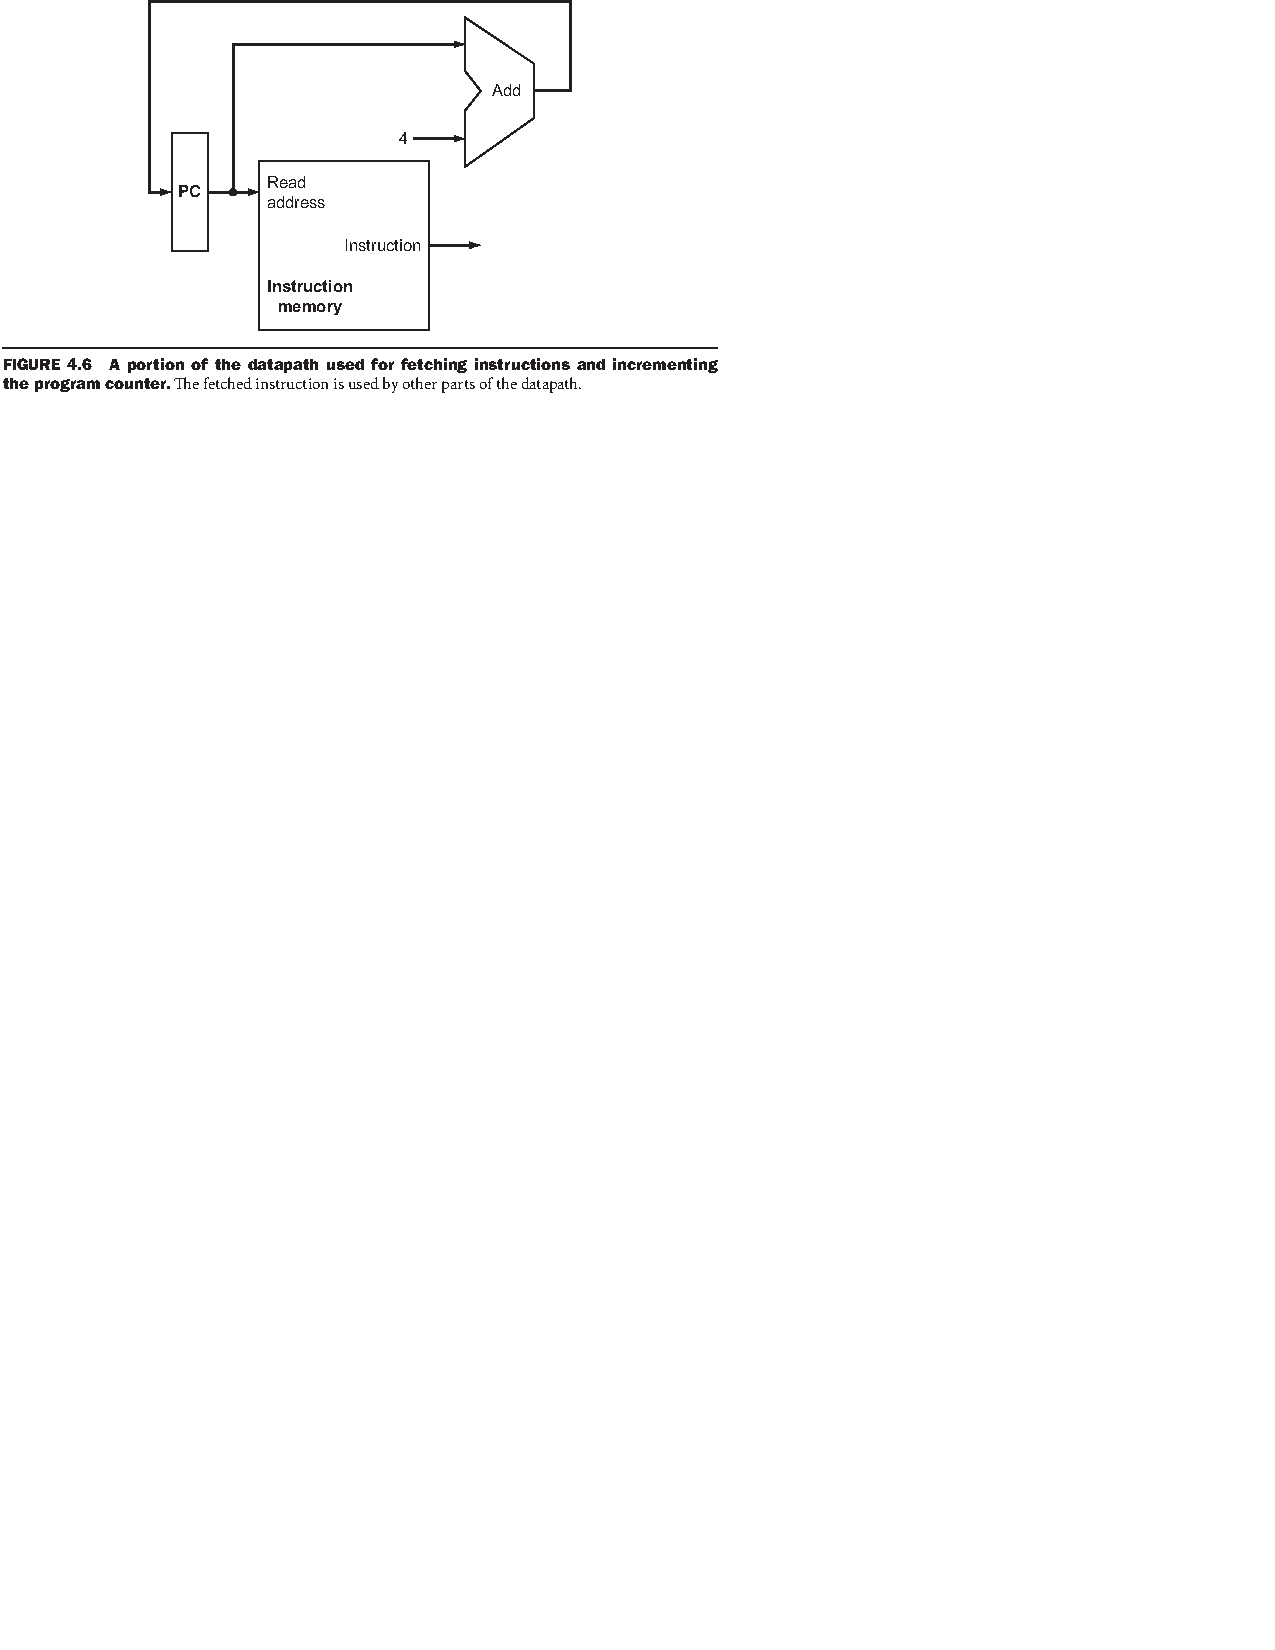
\includegraphics[width=\textwidth]{instruction.pdf}
    \caption{指令存储器}
    \label{fig:instr}
\end{figure}

指令存储器通过读取 PC 的值获取需要读取的指令地址。如果读取的内存地址越界,就读取第一个指令。

指令存储器被设定为 64 行。指令存储器的实现如下:

\begin{lstlisting}[caption=InstMemory.v]
module InstMemory(
    input [31:0] readAddress,
    output [31:0] inst
    );
    reg [31:0] instructions [0:63];
    assign inst = instructions[readAddress / 4 < 64 ? readAddress / 4 : 0];
endmodule
\end{lstlisting}

\subsection{顶层模块设计(一)}

\begin{figure}[H]
    \centering
    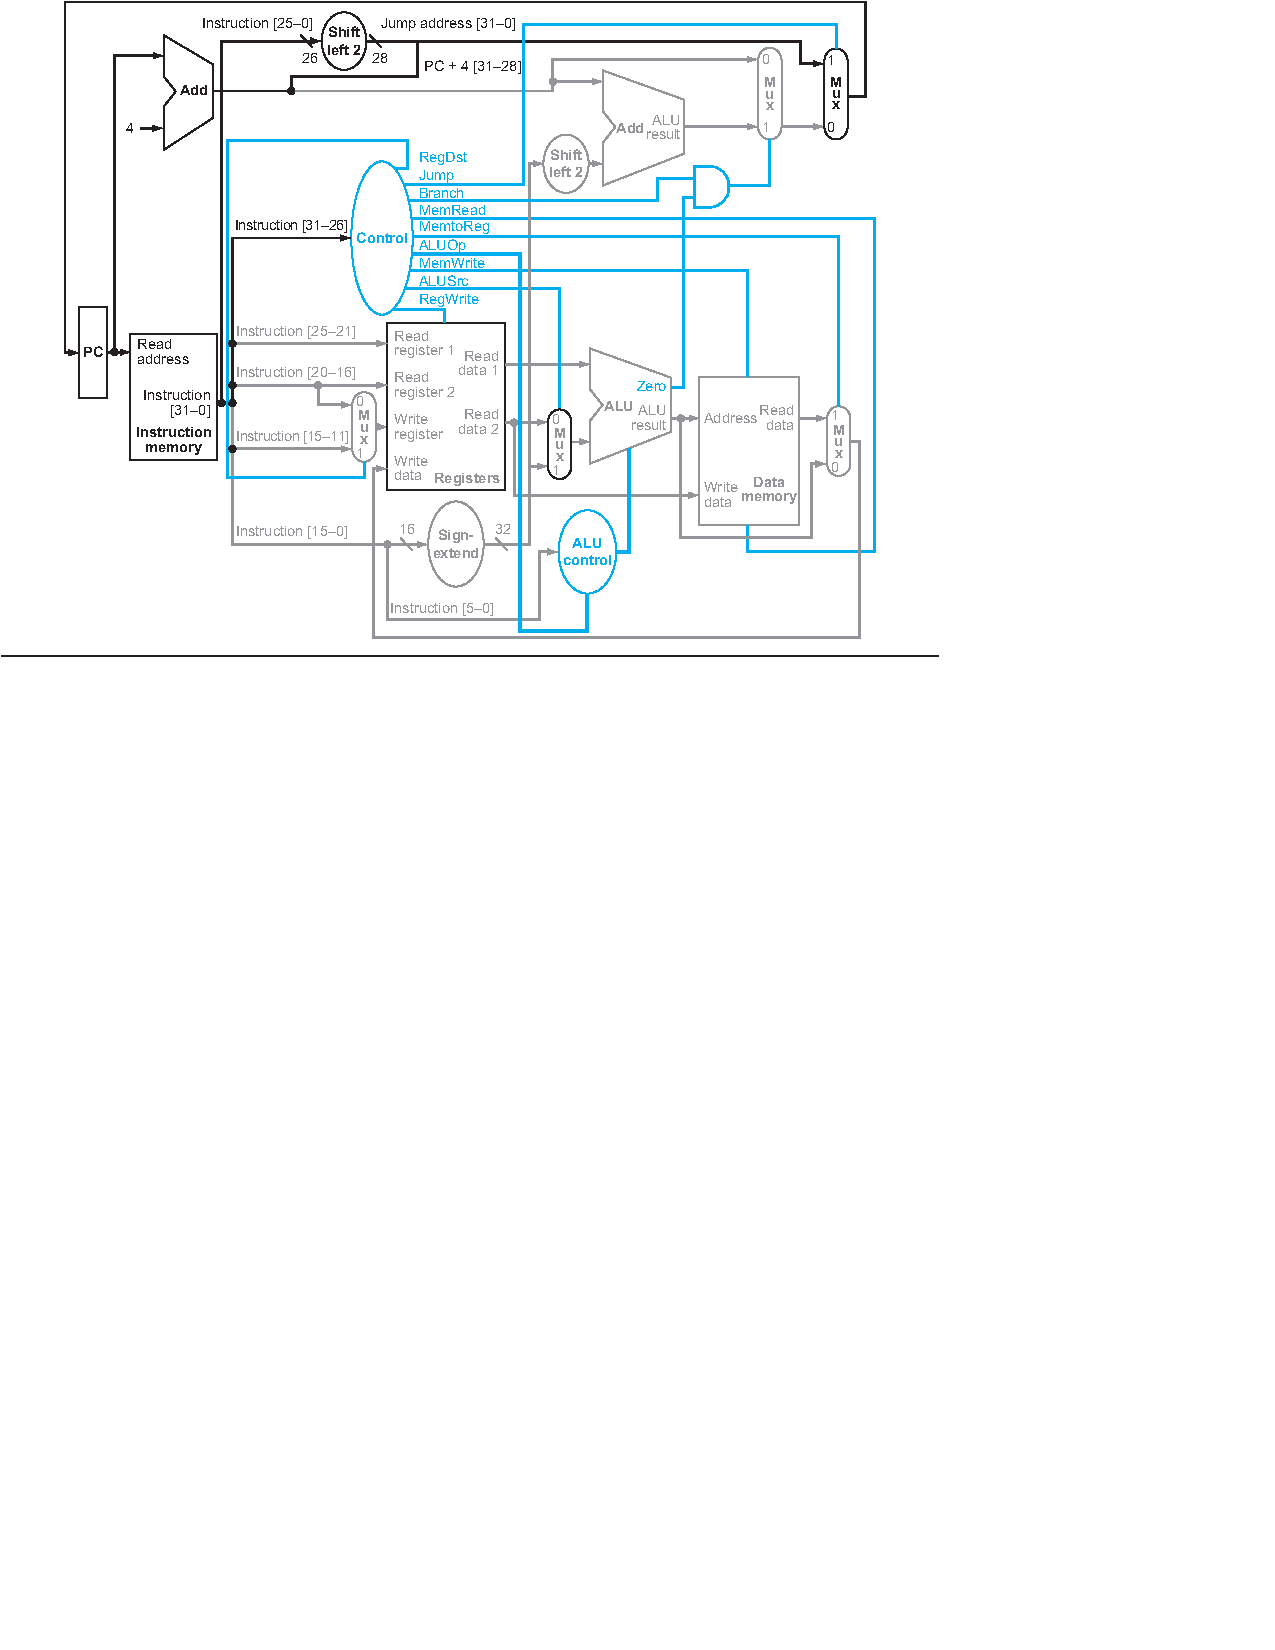
\includegraphics[width=\textwidth]{struct.pdf}
    \caption{顶层设计}
    \label{fig:top}
\end{figure}

单周期 MIPS 处理器共分为五个阶段:指令获取(IF)、指令译码(ID)、执行(EX)、存储(MEM)、写回(WB)。图 \ref{fig:top} 展示了针对 9 条指令的顶层模块设计。而针对 16 条指令,需要对一些原有的输入输出进行扩展。

\begin{table}[H]
    \centering
    \caption{16条指令}
    \begin{tabular}{>{\sffamily}c>{\sffamily}c>{\sffamily}c>{\sffamily}c}
        \hline
        add & sub & and & or \\
        \bfseries addi & \bfseries andi & \bfseries ori & slt \\
        lw & sw & \bfseries sll & \bfseries srl \\
        beq & j &\bfseries jal &\bfseries jr \\ 
        \hline
    \end{tabular}
\end{table}

\clearpage

\subsection{Ctr 扩展}

Ctr 模块会被扩展三个输出信号,相关信息如表 \ref{tab:Ctr} 和图 \ref{fig:Ctr} 所示。
\begin{table}[h]
    \centering
    \caption{Ctr 的扩展信号}\label{tab:Ctr}
    \begin{tabular}{>{\sffamily}cl>{\ttfamily}c>{\ttfamily}c}
        \toprule
        信号 & 描述 & 输出 & 输入\\
        \midrule
        zext & 是否为零扩展 & Ctr & sigext \\
        imm & 是否是立即数命令 & Ctr & ALUCtr \\
        jal & 是否是跳转链接命令 & Ctr & Registers \\
        \bottomrule
    \end{tabular}
\end{table}

\begin{figure}[h]
    \centering
    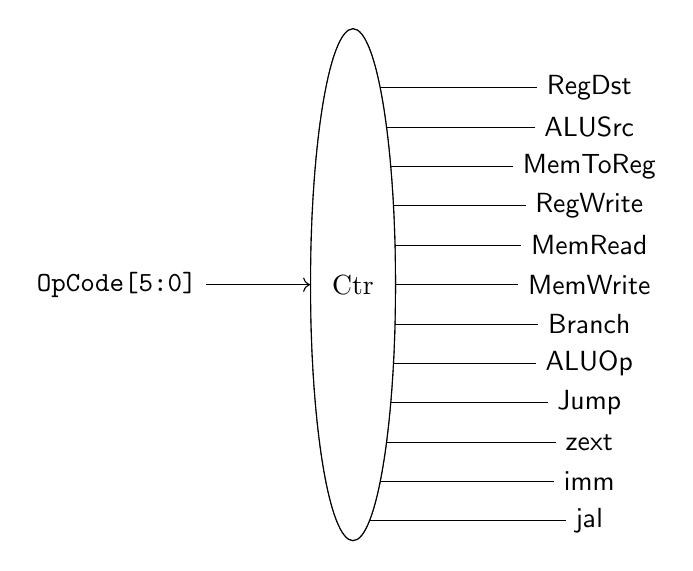
\begin{tikzpicture}

\node [ellipse,draw,minimum height=6.5cm,fill=white] (v2) at (0,0) {Ctr};
\node [font=\ttfamily] (v1) at (-3,0) {OpCode[5:0]};

\draw  (v1) edge[->] (v2);
\node[font=\sffamily] (v3) at (3,2.5) {RegDst};
\node[font=\sffamily] (v4) at (3,2) {ALUSrc};
\node[font=\sffamily] (v5) at (3,1.5) {MemToReg};
\node[font=\sffamily] (v6) at (3,1) {RegWrite};
\node[font=\sffamily] (v7) at (3,0.5) {MemRead};
\node[font=\sffamily] (v8) at (3,0) {MemWrite};
\node[font=\sffamily] (v9) at (3,-0.5) {Branch};
\node[font=\sffamily] (v10) at (3,-1) {ALUOp};
\node[font=\sffamily] (v11) at (3,-1.5) {Jump};
\node[font=\sffamily] (v12) at (3,-2) {zext};
\node[font=\sffamily] (v13) at (3,-2.5) {imm};
\node[font=\sffamily] (v14) at (3,-3) {jal};

\foreach \x in {3,...,14}
    \draw (v2) |- (v\x);

\node [ellipse,draw,minimum height=6.5cm,fill=white] at (0,0) {Ctr};


\end{tikzpicture}
    \caption{扩展端口后的 Ctr}
    \label{fig:Ctr}
\end{figure}

扩展信号输出后就可以支持 \textsf{addi}, \textsf{andi}, \textsf{ori}, \textsf{jal} ,在实验 3 表 2 的基础上扩增:
\begin{table}[H]
    \centering
    \caption{增扩指令}
    \begin{tabular}{>{\sffamily}c>{\ttfamily}c>{\ttfamily}c>{\ttfamily}c>{\ttfamily}c}
        \toprule
        信号 & addi & andi & ori & jal \\
        \midrule
        zext & 0 & 1 & 1 & 0\\
        imm & 1 & 1 & 1 & 0\\
        jal & 0 & 0 & 0 & 1\\
        \bottomrule
    \end{tabular}
\end{table}
\clearpage
\subsection{ALUCtr 扩展}

针对 ALUCtr 也会进行信号扩增,如表 \ref{tab:aluctr} 和图 \ref{fig:aluctr} 所示。
\begin{table}[h]
    \centering
    \caption{ALUCtr 的扩展信号}\label{tab:aluctr}
    \begin{tabular}{>{\sffamily}cl>{\ttfamily}c>{\ttfamily}c}
        \toprule
        信号 & 描述 & 输出 & 输入\\
        \midrule
        nop & 是否为空指令 & InstMemory & ALUCtr \\
        jr & 是否为跳转寄存器指令 & ALUCtr & PC \\
        shamt & ALU第一个信号是否是 shamt 位 & ALUCtr & ALU \\
        \bottomrule
    \end{tabular}
\end{table}

\begin{figure}[h]
    \centering
    \begin{tikzpicture}

\node [ellipse,draw,minimum height=3cm,fill=white] (v2) at (0,0) {ALUCtr};
\node [font=\ttfamily] (v1) at (-3,0) {funct[5:0]};
\node [font=\sffamily] (v3) at (0,-3) {ALUOp[1:0]};
\node [font=\sffamily] (v4) at (3,0) {aluCtrOut[3:0]};
\node [font=\ttfamily] (v5) at (-3,1) {nop};
\node [font=\sffamily] (v6) at (-0.5,3.5) {jr};
\node [font=\sffamily] (v7) at (0.5,3.5) {shamt};

\draw (v1) edge[->] (v2);
\draw (v3) edge[->] (v2);
\draw (v2) edge[->] (v4);
\draw (v5) -| (v2.center);
\draw [->] (v2) -| (v6);
\draw [->] (v2) -| (v7);

\node [ellipse,draw,minimum height=3cm,fill=white] (v2) at (0,0) {ALUCtr};
\end{tikzpicture}
    \caption{扩展端口后的 ALUCtr}
    \label{fig:aluctr}
\end{figure}

添加 \verb"nop" 信号是因为其指令与 \verb"sll" 冲突,如表 \ref{tab:inst} 所示。

\begin{table}[H]
    \centering
    \caption{增广指令}\label{tab:inst}
    \begin{tabular}{>{\sffamily}c>{\ttfamily}c>{\ttfamily}c>{\ttfamily}c>{\ttfamily}c>{\ttfamily}c>{\ttfamily}c|>{\ttfamily}c}
        \toprule
        指令 & op & rs & rt & rd & shamt & funct & ALUCtrOut \\
        \midrule
        nop & 000000 & 00000 & 00000 & 00000 & 00000 & 000000 & 1111\\
        sll & 000000 & 00000 & rt & rd & shamt & 000000 & 1000\\
        srl & 000000 & 00000 & rt & rd & shamt & 000010 & 1001\\
        jr & 000000 & rs & 00000 & 00000 & 00000 & 001000 & 1111\\
        \bottomrule
    \end{tabular}
\end{table}

\subsection{跳转与PC}

本处理器为统一起见,将时钟上跳沿设定为取指和递增,下跳沿将会处理跳转与分支相关的指令。示意图如图 \ref{fig:jr} 所示。

\begin{figure}[H]
    \centering
    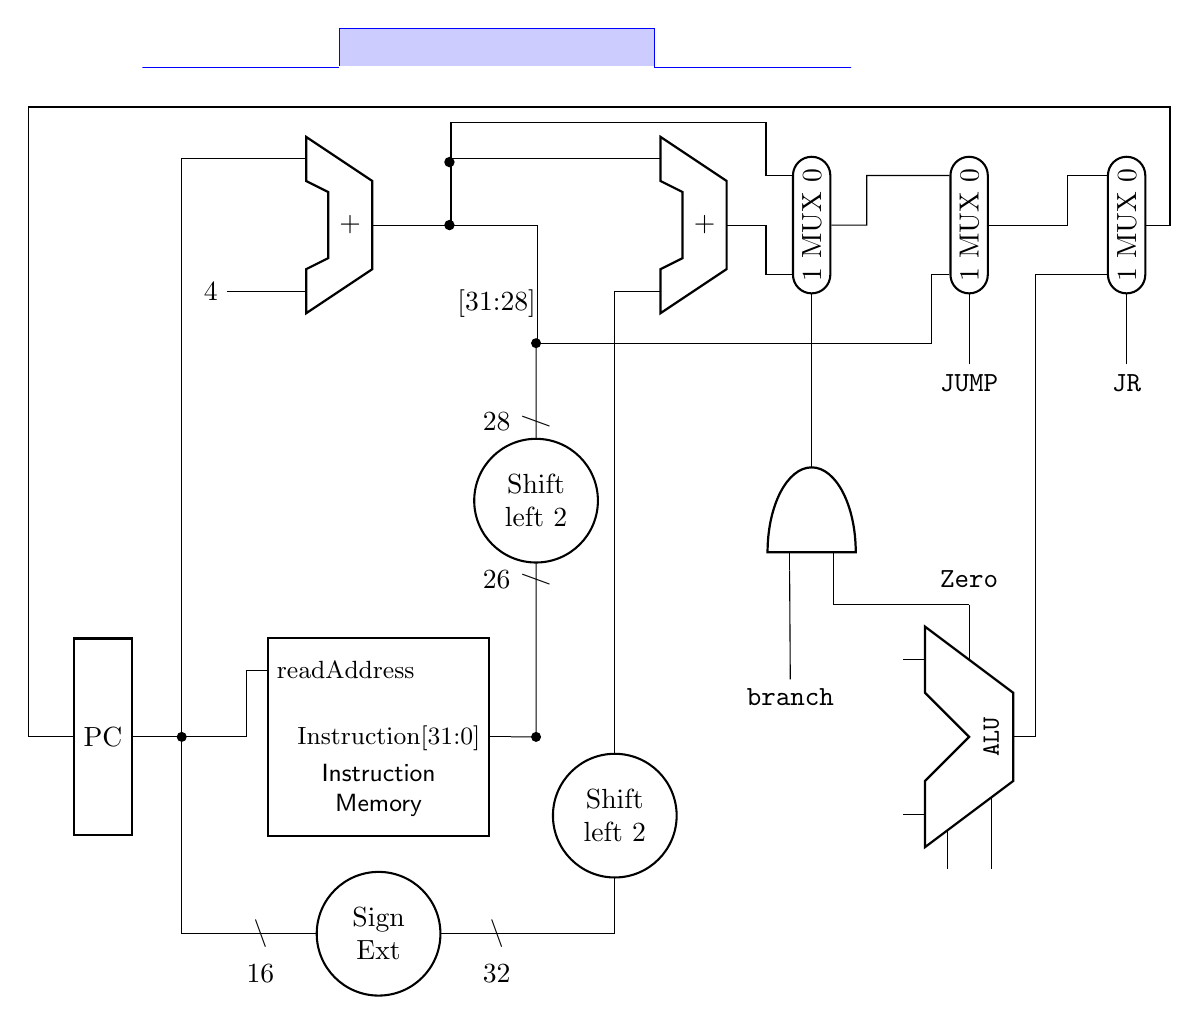
\begin{tikzpicture}
\ctikzset{multipoles/dipchip/width=2, multipoles/flipflop/width=2}
\tikzstyle{element} = [flipflop,text width=4.5em,text centered,font=\small\sffamily];
\tikzstyle{mux} = [rounded rectangle,draw,rotate=90,line width=0.75pt];
\tikzstyle{sigext} = [line width=0.75pt,draw,fill=white,text width=3em,text centered,circle];
\node [ALU] (exALU) at (3,-1.5) {{\rotatebox{90}{\small \ttfamily ALU}}};
%\node [element,] (PC) at (-9.5,-1.5) {PC};
\node [draw,minimum height=2.5cm,line width=0.75pt] (PC) at (-8,-1.5) {PC};
\node [element,flipflop def={t1=readAddress,t5=Instruction[31:0]},text height=4.5em] (Inst) at (-4.5,-1.5) {Instruction Memory};
\draw (PC.east) to[short,-*] (-7,-1.5) -| (Inst.pin 1);
\draw (Inst.pin 5) to[short,-*] (-2.5,-1.5) node (v8) {} to[short,-*] (-2.5,3.5) node (v9) {};

%\node [dipchip, hide numbers, no topmark, external pins width=0,font=\small\sffamily] (Reg) at (2,-5.5) {Registers};
%\node [right] at (Reg.bpin 1) {readReg1};
%\node [right] at (Reg.bpin 2) {readReg2};
%\node [right] at (Reg.bpin 3) {writeReg};
%\node [right] at (Reg.bpin 4) {writeData};

\node [one bit adder,external pins width=0] (oALU) at (-5,5) {+};
\draw (-7,-1.5) node (v13) {} |- (oALU.lpin 1);
\node [left, xshift=-1cm] (v4) at (oALU.lpin 2){4};
\draw (v4) -- (oALU.lpin 2);

\draw[fill=blue!20,draw=blue] (-7.5,7) -- (-5,7) node (v1) {} -- (-5,7.5) -- (-1,7.5) -- (-1,7) node (v2) {} -- (1.5,7) -- cycle;
\draw[draw=white,line width=1pt]  (-5,7) edge (-1,7);
\node[mux] (v5) at (5,5) {1 MUX 0};
\node[font=\ttfamily] (v3) at (5,3) {JR};
\draw  (v3) edge (v5);
\draw (exALU.rpin 1) |- (v5.north west);
\node [mux] (v7) at (3,5) {1 MUX 0};
\draw (v5.south) -- ++(right:3mm) -- ++(0,1.5) --++ (-14.5,0) |- (PC.west);

\node[font=\ttfamily] (v6) at (3,3) {JUMP};
\draw  (v6) edge (v7);
\draw (v7.south) -- ++(right:10mm) |- (v5.north east);
\draw (oALU.rpin 1) --++(2.1,0) --++ (0,-1.5) --++(5,0) |- (v7.north west);

\node at (-3,0.5) {26};
\node[rotate=90] at (-2.5,0.5) {$\slash$};
\node at (-3,4) {[31:28]};
\node[sigext] at (-2.5,1.5) {Shift left 2};
\node[rotate=90] at (-2.5,2.5) {$\slash$};
\node at (-3,2.5) {28};

\node[and port,rotate=90] (and) at (1,2) {};
\draw (exALU.tpin 1) -| (and.in 2);
\node[font=\ttfamily] (v10) at (0.73,-1) {branch};
\draw  (v10) edge (and.in 1);
\node [mux] (v11) at (1,5) {1 MUX 0};
\draw (and.out) |- (v11.west);
\draw  (v11) --++(0.7,0) |- (v7.north east);
\draw (oALU.rpin 1) --++ (right:10mm) --++(0,1.3) --++(4,0) |- (v11.north east);
\node [sigext] (v12) at (-4.5,-4) {Sign Ext};


\node[one bit adder,external pins width=0] (oALUo) at (-0.5,5) {+};
\draw  (oALUo.rpin 1) --++(right:5mm) |- (v11.north west);

\draw  (v12) --++(3,0) |- (oALUo.lpin 2);
\node [sigext] at (-1.5,-2.5) {Shift left 2};
\draw  (oALU.rpin 1) --++(right:10mm) |- (oALUo.lpin 1);
\node[fill,circle,scale=0.4] at (-3.6,5) {};
\node[fill,circle,scale=0.4] at (-3.6,5.8) {};
\draw  (-7,-1.5) |- (v12);
\node at (-3,-4) {$\backslash$};
\node at (-6,-4) {$\backslash$};
\node at (-6,-4.5) {16};
\node at (-3,-4.5) {32};
\node[font=\ttfamily] at (3,0.5) {Zero};

\end{tikzpicture}
    \caption{跳转与 PC}
    \label{fig:jr}
\end{figure}

% 上跳沿相关的指令:
\begin{lstlisting}
    always @(posedge clk) begin
        if(reset) PC <= 0; else  PC <= PC + 4; end
    InstMemory instMemory(.readAddress(PC), .inst(INST));
\end{lstlisting}

% 下跳沿相关的指令:
\begin{lstlisting}
    always @(negedge clk) begin
        PC <= JR ? ALU_RES : (JUMP ? (PC[31:28] + INST[25:0] << 2) : 
                    ((BRANCH & ZERO) ? (PC + (OPRAND << 2)) : PC)); end
\end{lstlisting}

\subsection{JAL 和寄存器堆}

Jump And Link (JAL) 指令会影响寄存器堆的输入。如图 \ref{fig:jal} 所示,在有 JAL 指令时会直接写入第 31 号寄存器,并写入 PC + 4 的值(此时 PC 还没有变化,保留上一次末尾值)。

\begin{figure}[h]
    \centering
    \usetikzlibrary{shapes.misc}
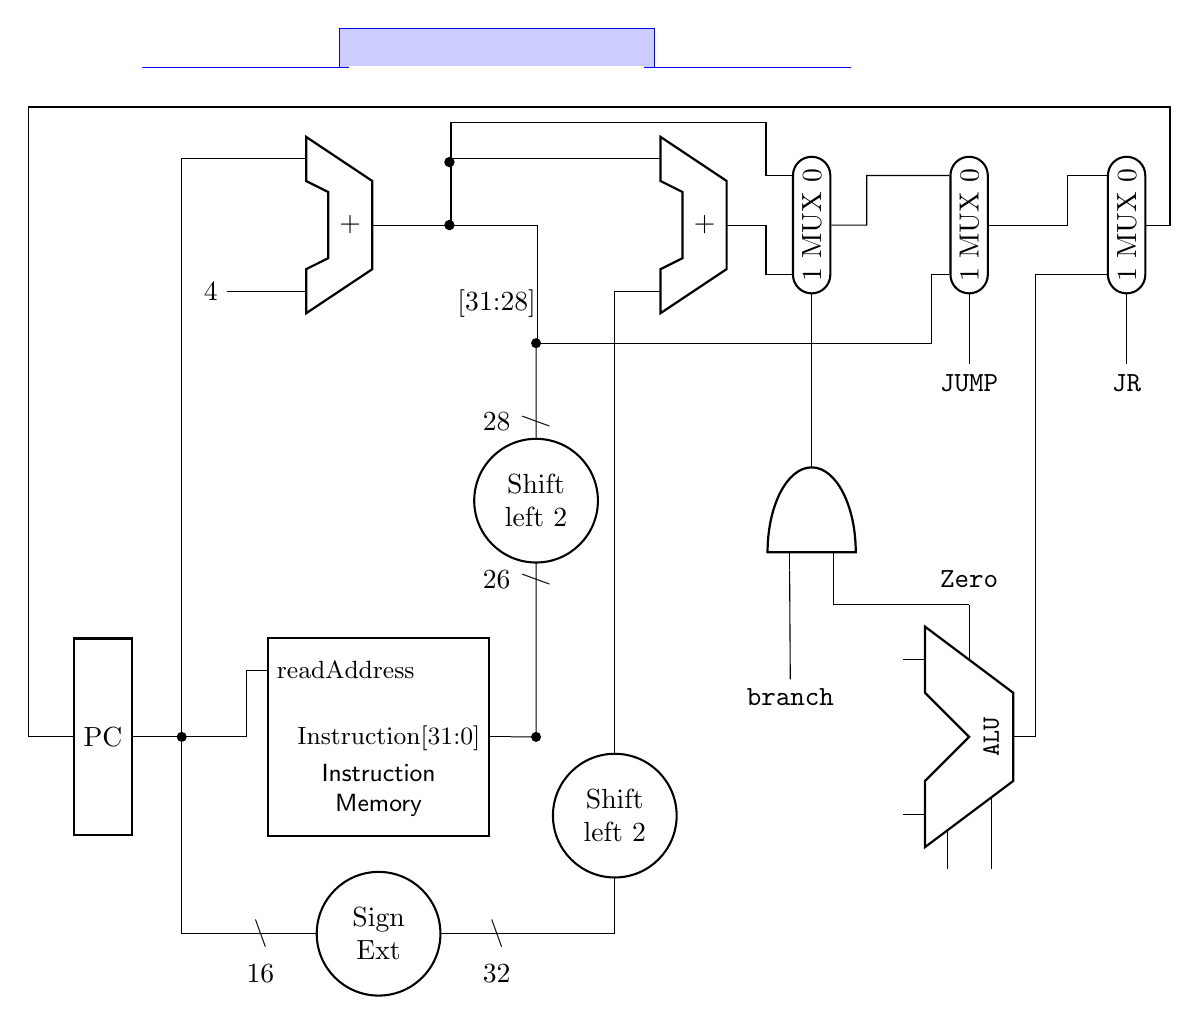
\begin{tikzpicture}
\ctikzset{multipoles/dipchip/width=2, multipoles/flipflop/width=2}
\tikzstyle{element} = [flipflop,text width=4.5em,text centered,font=\small\sffamily];
\tikzstyle{mux} = [rounded rectangle,draw,rotate=90,line width=0.75pt];
\tikzstyle{sigext} = [line width=0.75pt,draw,fill=white,text width=3em,text centered,circle];
\node [ALU] (exALU) at (3,-1.5) {{\rotatebox{90}{\small \ttfamily ALU}}};
%\node [element,] (PC) at (-9.5,-1.5) {PC};
\node [draw,minimum height=2.5cm,line width=0.75pt] (PC) at (-8,-1.5) {PC};
\node [element,flipflop def={t1=readAddress,t5=Instruction[31:0]},text height=4.5em] (Inst) at (-4.5,-1.5) {Instruction Memory};
\draw (PC.east) to[short,-*] (-7,-1.5) -| (Inst.pin 1);
\draw (Inst.pin 5) to[short,-*] (-2.5,-1.5) node (v8) {} to[short,-*] (-2.5,3.5) node (v9) {};

%\node [dipchip, hide numbers, no topmark, external pins width=0,font=\small\sffamily] (Reg) at (2,-5.5) {Registers};
%\node [right] at (Reg.bpin 1) {readReg1};
%\node [right] at (Reg.bpin 2) {readReg2};
%\node [right] at (Reg.bpin 3) {writeReg};
%\node [right] at (Reg.bpin 4) {writeData};

\node [one bit adder,external pins width=0] (oALU) at (-5,5) {+};
\draw (-7,-1.5) node (v13) {} |- (oALU.lpin 1);
\node [left, xshift=-1cm] (v4) at (oALU.lpin 2){4};
\draw (v4) -- (oALU.lpin 2);

\draw[fill=blue!20,draw=blue] (-7.5,7) -- (-5,7) node (v1) {} -- (-5,7.5) -- (-1,7.5) -- (-1,7) node (v2) {} -- (1.5,7) -- cycle;
\draw[draw=white,line width=1pt]  (v1) edge (v2);
\node[mux] (v5) at (5,5) {1 MUX 0};
\node[font=\ttfamily] (v3) at (5,3) {JR};
\draw  (v3) edge (v5);
\draw (exALU.rpin 1) |- (v5.north west);
\node [mux] (v7) at (3,5) {1 MUX 0};
\draw (v5.south) -- ++(right:3mm) -- ++(0,1.5) --++ (-14.5,0) |- (PC.west);

\node[font=\ttfamily] (v6) at (3,3) {JUMP};
\draw  (v6) edge (v7);
\draw (v7.south) -- ++(right:10mm) |- (v5.north east);
\draw (oALU.rpin 1) --++(2.1,0) --++ (0,-1.5) --++(5,0) |- (v7.north west);

\node at (-3,0.5) {26};
\node[rotate=90] at (-2.5,0.5) {$\slash$};
\node at (-3,4) {[31:28]};
\node[sigext] at (-2.5,1.5) {Shift left 2};
\node[rotate=90] at (-2.5,2.5) {$\slash$};
\node at (-3,2.5) {28};

\node[and port,rotate=90] (and) at (1,2) {};
\draw (exALU.tpin 1) -| (and.in 2);
\node[font=\ttfamily] (v10) at (0.73,-1) {branch};
\draw  (v10) edge (and.in 1);
\node [mux] (v11) at (1,5) {1 MUX 0};
\draw (and.out) |- (v11.west);
\draw  (v11) --++(0.7,0) |- (v7.north east);
\draw (oALU.rpin 1) --++ (right:10mm) --++(0,1.3) --++(4,0) |- (v11.north east);
\node [sigext] (v12) at (-4.5,-4) {Sign Ext};


\node[one bit adder,external pins width=0] (oALUo) at (-0.5,5) {+};
\draw  (oALUo.rpin 1) --++(right:5mm) |- (v11.north west);

\draw  (v12) --++(3,0) |- (oALUo.lpin 2);
\node [sigext] at (-1.5,-2.5) {Shift left 2};
\draw  (oALU.rpin 1) --++(right:10mm) |- (oALUo.lpin 1);
\node[fill,circle,scale=0.4] at (-3.6,5) {};
\node[fill,circle,scale=0.4] at (-3.6,5.8) {};
\draw  (-7,-1.5) |- (v12);
\node at (-3,-4) {$\backslash$};
\node at (-6,-4) {$\backslash$};
\node at (-6,-4.5) {16};
\node at (-3,-4.5) {32};
\node[font=\ttfamily] at (3,0.5) {Zero};

\end{tikzpicture}
    \caption{JAL 和寄存器堆}
    \label{fig:jal}
\end{figure}

\begin{lstlisting}
    Registers registers(
        .clk(clk),
        .reset(reset),
        .readReg1(INST[25:21]),
        .readReg2(INST[20:16]),
        .writeReg(JAL ? 5'b11111 : (JR ? INST[25:21] : (REG_DST ? INST[15:11] : INST[20:16]))),
        .writeData(JAL ? PC + 4 : (MEM_TO_REG ? READ_DATA : ALU_RES)), // Jal will jump to PC + 4
        .regWrite(REG_WRITE),
        .readData1(READ_DATA1),
        .readData2(READ_DATA2)
    );
\end{lstlisting}

\subsection{顶层模块设计(二)}

添加这些数据线后,就可以支持 16 条指令了。

\begin{multicols}{2}
    \code{Top.v}{verilog}
\end{multicols}

% \section{代码实现}

% \subsection{指令存储器}

\section{仿真结果}

使用了下面的指令文件进行仿真。该指令文件主要的作用是测试所有的运算功能,并在每一个循环对 10 号寄存器 + 1,并存储到 0 号存储单元中,直到其超过刚开始的限制寄存器的存储数字(这里是 4),之后就会进入短循环,不会再对寄存器和存储器进行修改。

% \begin{multicols}{2}
    \code{simple.asm}{}
    \begin{lstlisting}[caption=mem\_data.mem]
00000001
00000001
00000004
00000000
00000000
00000000
00000000
00000000
00000000
    \end{lstlisting}
% \end{multicols}

激励文件加载指令集的时候,要注意 \verb"$readmemb" 是二进制读取,\verb"$readmemh" 是十六进制读取。

\begin{lstlisting}[caption=Basic\_tb.v]
module Basic_tb(

    );

    reg clk;
    reg reset;

    Top Proc(.clk(clk),.reset(reset));

    initial begin
        $readmemb("mem_inst.mem",Proc.instMemory.instructions);
        $readmemh("mem_data.mem",Proc.DataMemory.MemFile,10'h0);
        reset = 1;
        clk = 0;
    end

    always #10 clk = ~clk;

    initial begin
        #80 reset = 0;
    end

endmodule
\end{lstlisting}

\begin{figure}[H]
    \centering
    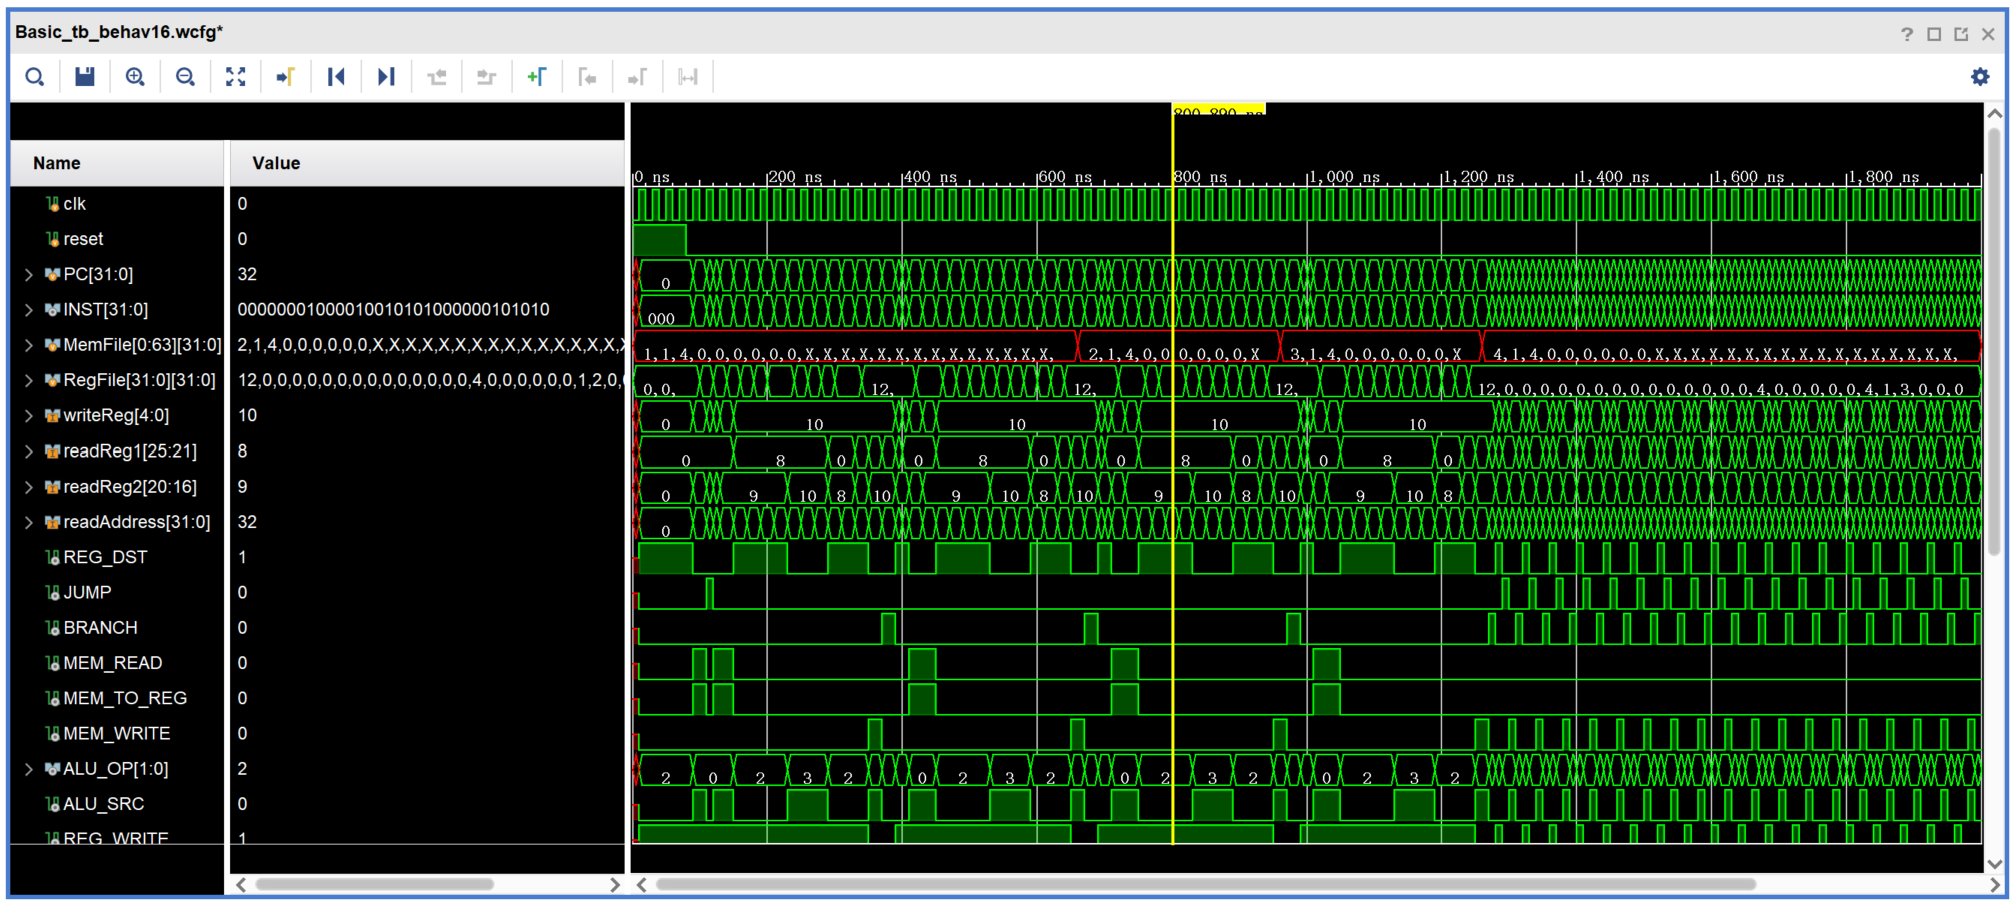
\includegraphics[width=\textwidth]{figure2.png}
    \caption{16条指令的仿真结果}
    \label{fig:16}
\end{figure}

运算细节见图 \ref{fig:calcde}。最后条件结束的情况见图 \ref{fig:cond}。所有的运算都得到了正确的结果。

\begin{figure}[H]
    \centering
    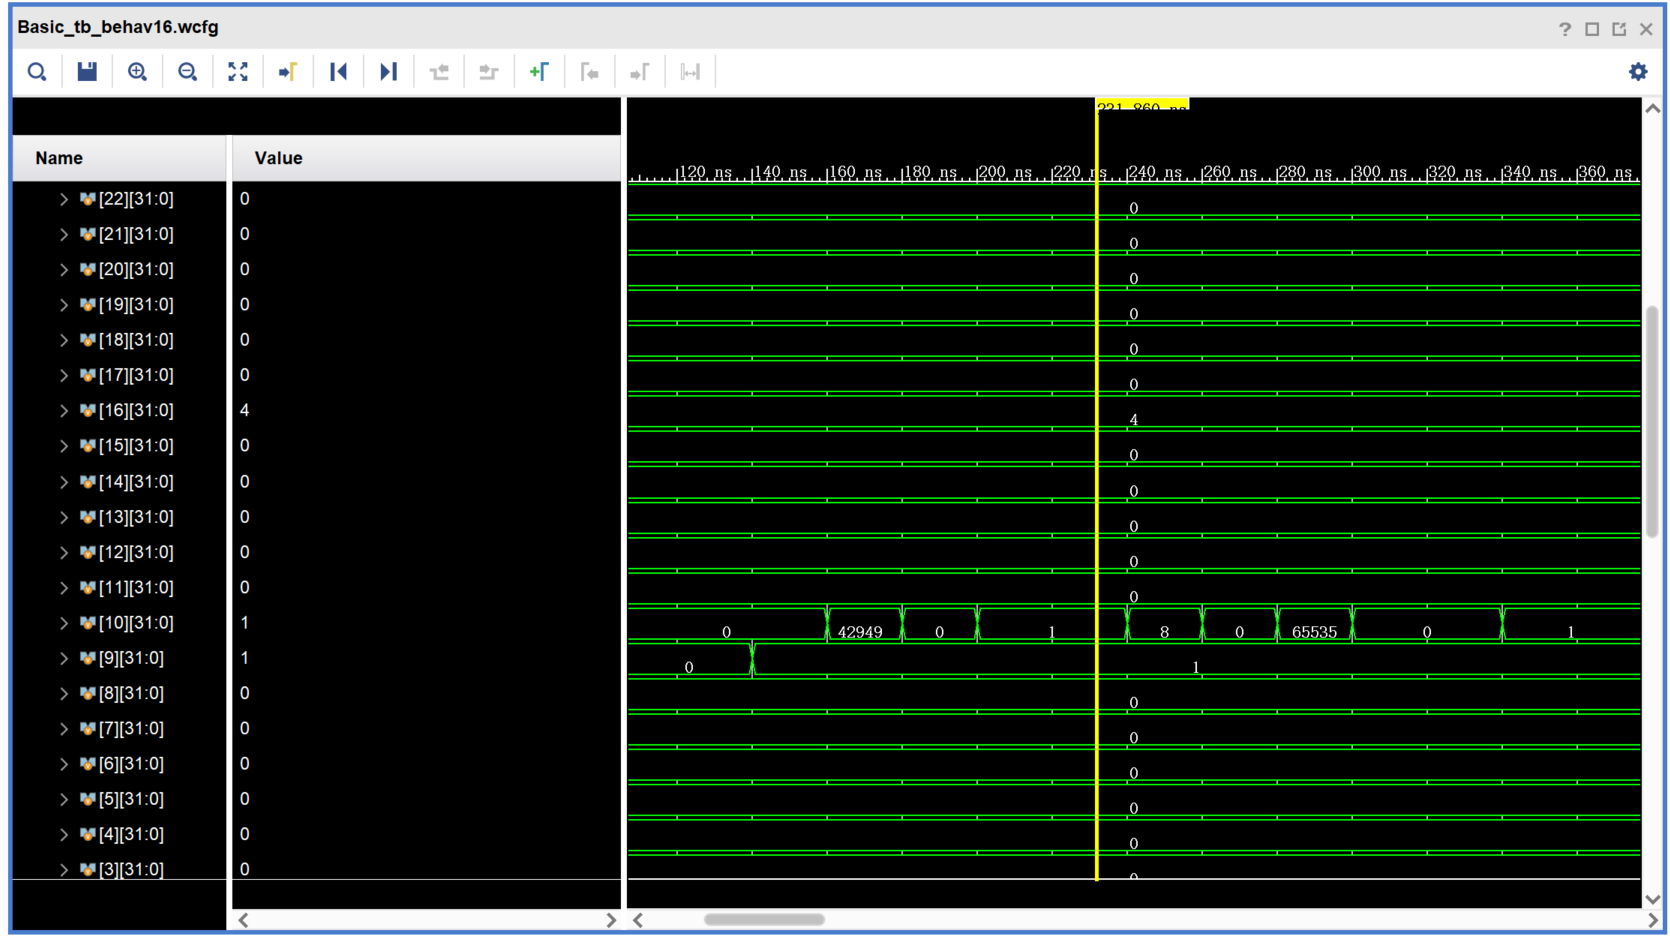
\includegraphics[width=\textwidth]{calcdetail.png}
    \caption{运算细节}
    \label{fig:calcde}
\end{figure}

\begin{figure}[H]
    \centering
    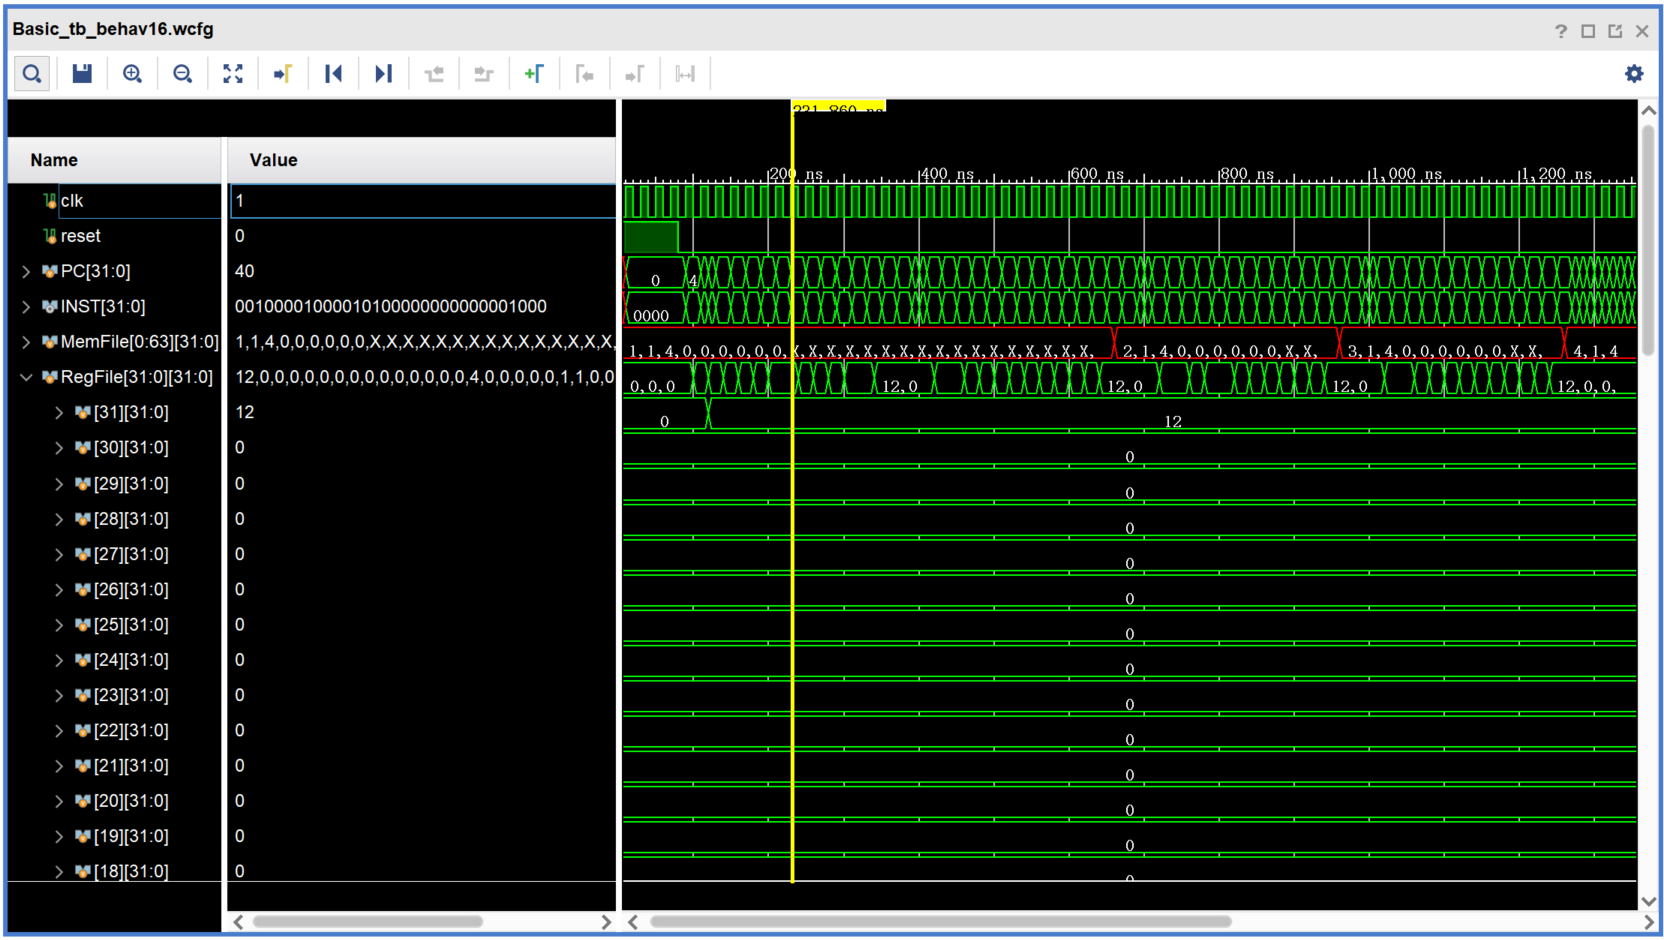
\includegraphics[width=\textwidth]{memdetail.png}
    \caption{最后条件结束}
    \label{fig:cond}
\end{figure}

\section{实验心得}

本次实验调试时间较长,花费近 8 个小时。

主要是顶层设计的连线方案比较复杂,对于增扩的指令,需要重新设计端口加以实现。查看波形进行逐个波形的调试,有助于排查故障。这里面对于 ALUCtr 使用了 nop 扩增非常关键,否则会导致空指令执行了某些移位操作导致 0 寄存器非零,从而影响下面数据的读取。对于 PC 的写入顺序进行了比较多的调试,最后确定了上跳沿递增、下跳沿跳转的方案,可以互不干扰。并且选路器没有采用模块化设计,而是使用三目运算符,让代码更加简洁易懂。

本次实验增加了我对单周期处理器设计的理解,对于理解一些原理有很大的帮助,对于下面的流水线处理器设计也会起到关键的作用。

\end{document}